\documentclass[11pt,a4paper]{article}
\usepackage[utf8]{inputenc}
\usepackage{amsmath,amsfonts,amssymb}
\usepackage{graphicx}
\usepackage{geometry}
\geometry{margin=1in}
\usepackage{booktabs}
\usepackage{hyperref}
\usepackage{float}
\usepackage{xcolor}

\title{\textbf{EE3621: Digital Signal Processing} \\ \Large Lecture 18: Wavelet Transform \& Multiresolution Analysis \\ \large (III B.Tech EEE)}
\author{Lecture Notes (40-Minute Plan)}
\date{}

\definecolor{darkbg}{HTML}{0d121f}
\definecolor{lighttext}{HTML}{e2e8f0}
\definecolor{primary}{HTML}{8b5cf6}
\definecolor{secondary}{HTML}{0dd5c5}

\pagecolor{darkbg}
\color{lighttext}

\hypersetup{
    colorlinks=true,
    linkcolor=secondary,
    urlcolor=secondary
}

\begin{document}

\maketitle

\section{Lecture Plan (40 Minutes Breakdown)}
\begin{itemize}
    \item \textbf{00:00 -- 07:00 (7 mins):} \textbf{Why Wavelets?} Limitations of STFT, time-frequency resolution trade-offs, and constant-Q analysis.
    \item \textbf{07:00 -- 14:00 (7 mins):} \textbf{Continuous Wavelet Transform (CWT):} Definition, mother wavelet, scaling and translation, admissibility condition.
    \item \textbf{14:00 -- 18:00 (4 mins):} \textbf{Common Mother Wavelets:} Haar, Morlet, Mexican Hat, Daubechies.
    \item \textbf{18:00 -- 25:00 (7 mins):} \textbf{Multiresolution Analysis (MRA):} Nested subspaces, scaling function, wavelet function, two-scale relations.
    \item \textbf{25:00 -- 32:00 (7 mins):} \textbf{Discrete Wavelet Transform (DWT):} Filter banks, Mallat's Algorithm, perfect reconstruction.
    \item \textbf{32:00 -- 37:00 (5 mins):} \textbf{Numerical Example:} Haar DWT of a 4-point signal.
    \item \textbf{37:00 -- 40:00 (3 mins):} \textbf{Applications \& Checkpoints:} JPEG 2000, ECG, Q\&A.
\end{itemize}

\noindent\rule{\textwidth}{0.5pt}

\section{Why Wavelets? The Limitations of STFT}
The Fourier Transform provides frequency content but loses time information. The Short-Time Fourier Transform (STFT) addresses this by multiplying the signal $x(t)$ with a sliding window $w(t)$:
\begin{equation}
X(t, \omega) = \int_{-\infty}^{\infty} x(\tau) w(\tau - t) e^{-j\omega \tau} d\tau
\end{equation}

\textbf{Physical Intuition:} A narrow window provides excellent time resolution but poor frequency resolution. A wide window provides excellent frequency resolution but poor time resolution. In STFT, the window size is fixed, so resolution is the same at all frequencies. Wavelets solve this using \textbf{constant-Q analysis}: narrow windows at high frequencies (for transients) and wide windows at low frequencies (for slow drifts).

\section{Continuous Wavelet Transform (CWT)}
The CWT is defined as:
\begin{equation}
W_x(a,b) = \frac{1}{\sqrt{|a|}} \int_{-\infty}^{\infty} x(t)\psi^*\left(\frac{t-b}{a}\right)dt
\end{equation}
Where $\psi(t)$ is the mother wavelet, $a > 0$ is the scale, and $b$ is the translation.

For the inverse transform to exist, $\psi(t)$ must satisfy the \textbf{admissibility condition}:
\begin{equation}
C_\psi = \int_0^\infty \frac{|\Psi(\omega)|^2}{\omega}d\omega < \infty
\end{equation}

\textbf{Theorem: Zero Mean Property}\\
If $C_\psi < \infty$ and $\Psi(\omega)$ is continuous at $\omega = 0$, then $\Psi(0) = 0$.

\textit{Proof:}
Assume $\Psi(0) = c \neq 0$. As $\omega \to 0$, $|\Psi(\omega)|^2 \to |c|^2$. The integrand becomes $\frac{|c|^2}{\omega}$, and $\int_0^\epsilon \frac{|c|^2}{\omega} d\omega \to \infty$, violating $C_\psi < \infty$. Thus, $\Psi(0) = 0$.

\section{Common Mother Wavelets}
\begin{itemize}
    \item \textbf{Haar Wavelet:} Simplest, a step function. Good for transitions.
    \item \textbf{Morlet Wavelet:} $\psi(t) = e^{-t^2/2}e^{j\omega_0 t}$. Modulated Gaussian, optimal joint time-frequency resolution.
    \item \textbf{Mexican Hat:} $\psi(t) = -\frac{d^2}{dt^2}e^{-t^2/2}$. Second derivative of a Gaussian, used in edge detection.
    \item \textbf{Daubechies:} Compactly supported orthogonal wavelets, used in compression.
\end{itemize}

\section{Multiresolution Analysis (MRA)}
MRA defines nested subspaces $V_j$:
\begin{equation}
\dots \subset V_2 \subset V_1 \subset V_0 \subset V_{-1} \subset \dots
\end{equation}
A scaling function $\phi(t)$ spans $V_0$. The wavelet function $\psi(t)$ spans the orthogonal complement $W_0$, where $V_{-1} = V_0 \oplus W_0$.

This leads to the \textbf{two-scale relations}:
\begin{align}
\phi(t) &= \sqrt{2}\sum_{k} h_0[k]\phi(2t-k) \\
\psi(t) &= \sqrt{2}\sum_{k} h_1[k]\phi(2t-k)
\end{align}

\section{Discrete Wavelet Transform (DWT)}
The DWT uses a filter bank. The signal is passed through lowpass $H_0$ and highpass $H_1$, then downsampled by 2 to yield approximation $cA$ and detail $cD$.
The Quadrature Mirror Filter (QMF) relation is:
\begin{equation}
h_1[k] = (-1)^k h_0[N-1-k]
\end{equation}
Mallat's algorithm iteratively applies this to $cA$. A $J$-level DWT yields $J+1$ subbands.

\subsection{Perfect Reconstruction}
The synthesis filter bank conditions for Perfect Reconstruction (PR) are:
\begin{align}
G_0(z)H_0(-z) + G_1(z)H_1(-z) &= 0 \quad (\text{Alias Cancellation}) \\
G_0(z)H_0(z) + G_1(z)H_1(z) &= 2z^{-L} \quad (\text{Distortion-free})
\end{align}

\begin{figure}[H]
\centering
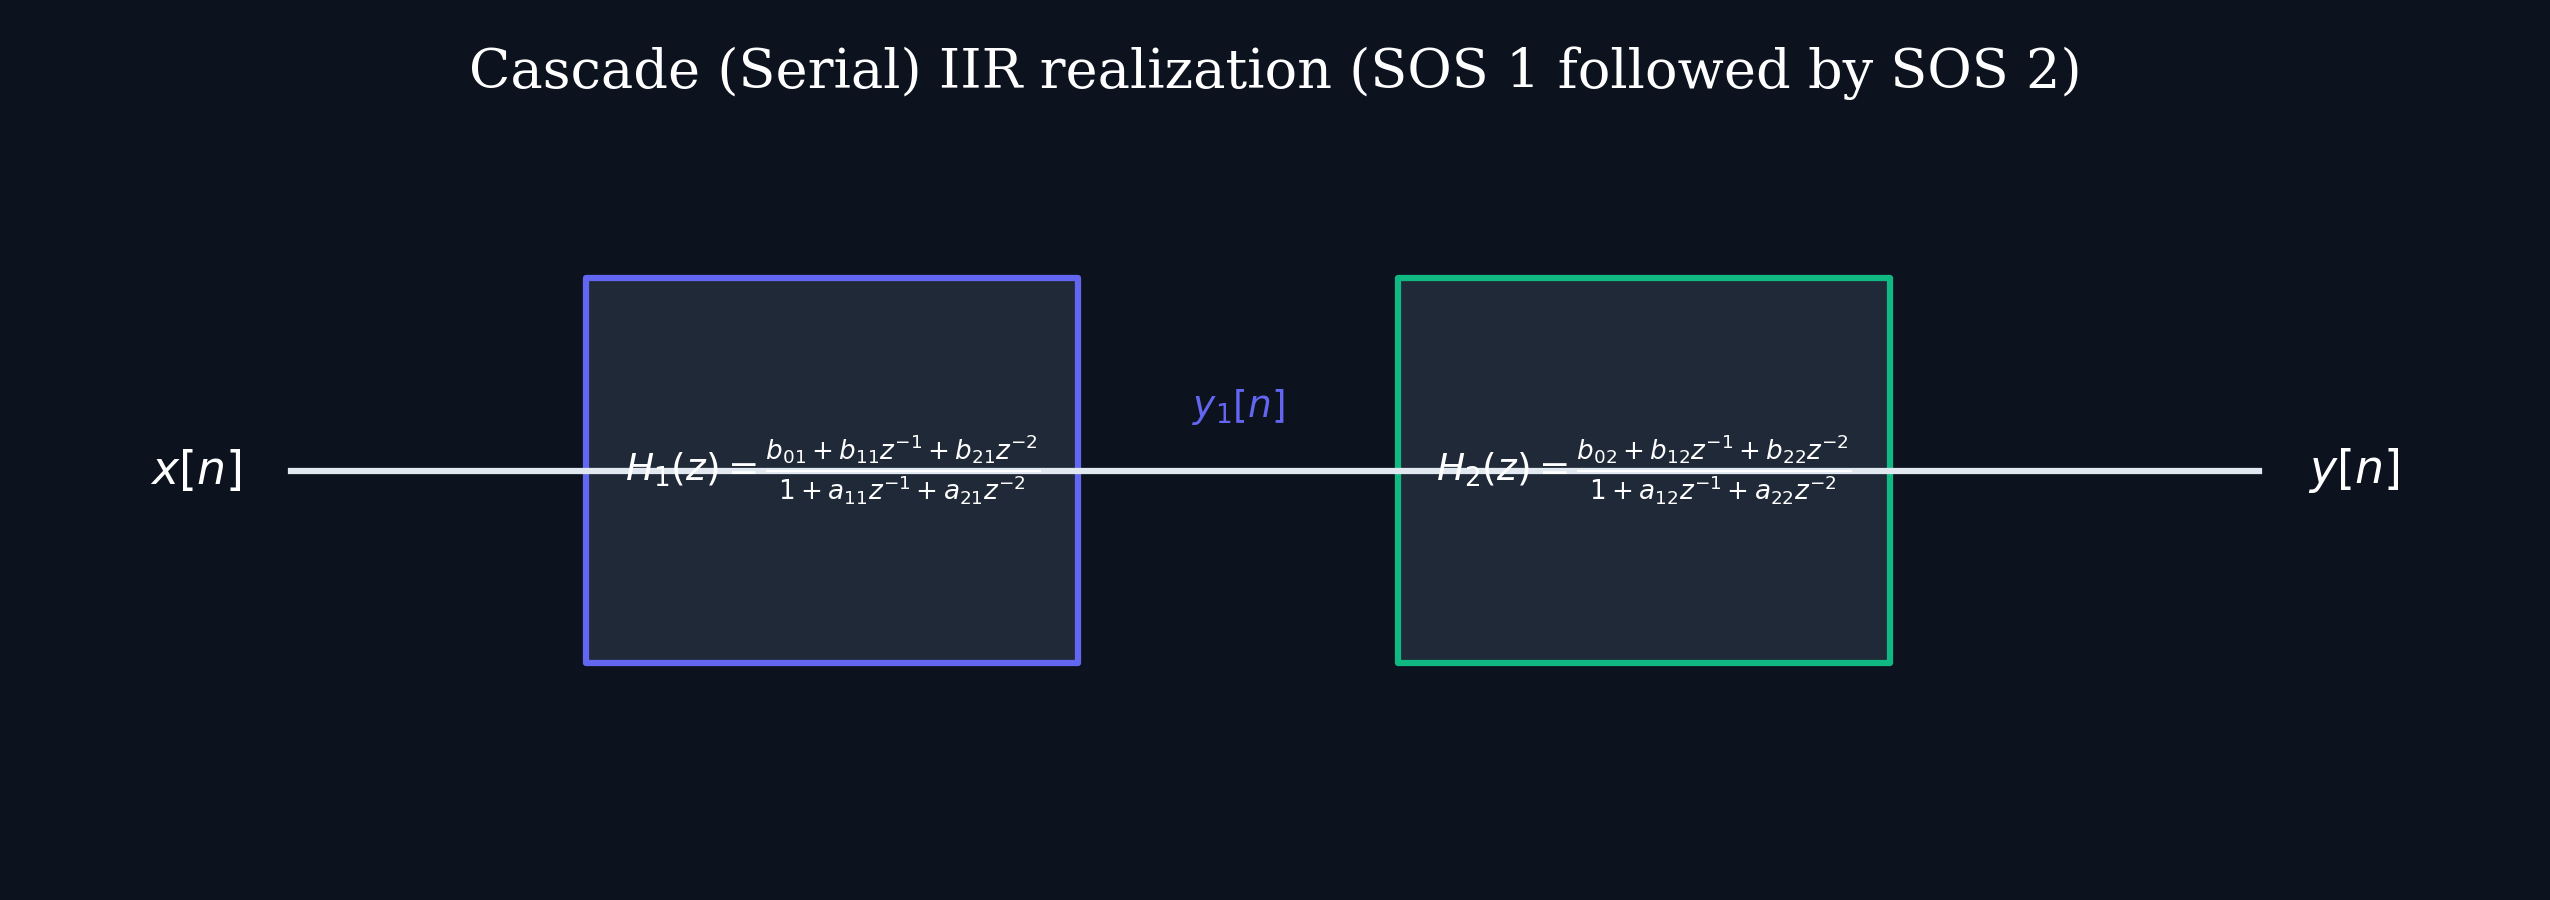
\includegraphics[width=0.7\textwidth]{images/iir_cascade.png}
\caption{Iterated cascade structure loosely analogous to DWT cascading filter stages.}
\label{fig:cascade}
\end{figure}

\section{Numerical Example: Haar DWT}
1-level Haar DWT of $x = [4, 6, 8, 2]$ using $h_0 = \frac{1}{\sqrt{2}}[1,1], h_1 = \frac{1}{\sqrt{2}}[1,-1]$.

\textbf{Approximation $cA$:}
\begin{align*}
cA[0] &= 4\left(\frac{1}{\sqrt{2}}\right) + 6\left(\frac{1}{\sqrt{2}}\right) = 5\sqrt{2} \\
cA[1] &= 8\left(\frac{1}{\sqrt{2}}\right) + 2\left(\frac{1}{\sqrt{2}}\right) = 5\sqrt{2}
\end{align*}

\textbf{Detail $cD$:}
\begin{align*}
cD[0] &= 4\left(\frac{1}{\sqrt{2}}\right) + 6\left(-\frac{1}{\sqrt{2}}\right) = -\sqrt{2} \\
cD[1] &= 8\left(\frac{1}{\sqrt{2}}\right) + 2\left(-\frac{1}{\sqrt{2}}\right) = 3\sqrt{2}
\end{align*}

\section{Applications}
\begin{itemize}
    \item \textbf{Image Compression:} JPEG 2000 uses DWT avoiding blocking artifacts.
    \item \textbf{ECG Denoising:} Thresholding DWT details to remove noise.
    \item \textbf{Seismic \& Edge Detection.}
\end{itemize}

\section{Checkpoints}
\begin{enumerate}
    \item \textbf{Why STFT struggles?} Fixed window width causes a rigid time-frequency trade-off. Wavelets solve this with variable windows.
    \item \textbf{Proof of zero mean:} If mean $\neq 0$, $\Psi(0) \neq 0$. The admissibility integral $\int \frac{|\Psi|^2}{\omega}$ would diverge at $\omega=0$.
    \item \textbf{3-level DWT subbands:} Yields 4 subbands: $cD_1, cD_2, cD_3, cA_3$.
\end{enumerate}

\end{document}
